\chapter{Ergebnisse}
\label{ch:results}

In diesem Kapitel werden die Ergebnisse der in \autoref{subsec:experimente} beschriebenen Experimente vorgestellt.
Zunächst wird beschrieben wie die Modelle, die mit teils verschieden langer Clips trainiert wurden, einheitlich verglichen werden können.
Anschließend werden die Ergebnisse aller vier Phasen vorgestellt.
Die Evaluation endet mit einer Kategorisierung der Klassen in vier Schwierigkeitsgrade und einer Einschätzung welchen Grenzen das Training unterlag.

\section{Vergleichbarkeit der Ergbnisse}

In den folgenden Abschnitten werden die Rechenergebnisse verschiedener Modelle verglichen.
Die Modelle unterscheiden sich, wie schon in \autoref{tab:coverage} gezeigt, durch verschiedene Hyperparameter, die zu verschiedenen Werten der Clip-Abdeckung $\Delta$ führen.
Während des Trainings werden im Trainings- und Validierungsset Samples generiert, die genau der Länge $\Delta$ entsprechen.
Das Test-Set umfasst wiederum stets die gleichen Samples mit einer Clip-Abdeckung von $\Delta=10$.
Die Test-Samples sind damit immer etwas oder sogar deutlich länger als Trainings- und Validierungssamples.

Während der Evaluation wird ein Clip vom Testsets in fünf Chunks segmentiert, die sich gleichmäßig über die komplette Clip-Länge verteilen und potentiell überschneiden.
Die Chunks werden einzeln inferiert und der endgültigen Score pro Clip ergibt sich aus einer Aggregation (consensus function) pro Klasse über allen Chunks.
Als Aggregation wurden in diesem Zusammenhang das Maximum und der Durchschnitt pro Klasse ermittelt.
\autoref{fig:consensus} zeigt einen exemplarischen Vergleich, der in diesem Zusammenhang repräsentativ für alle durchgeführten Experimente ist:

\begin{figure}[htbp!]
    \centering
    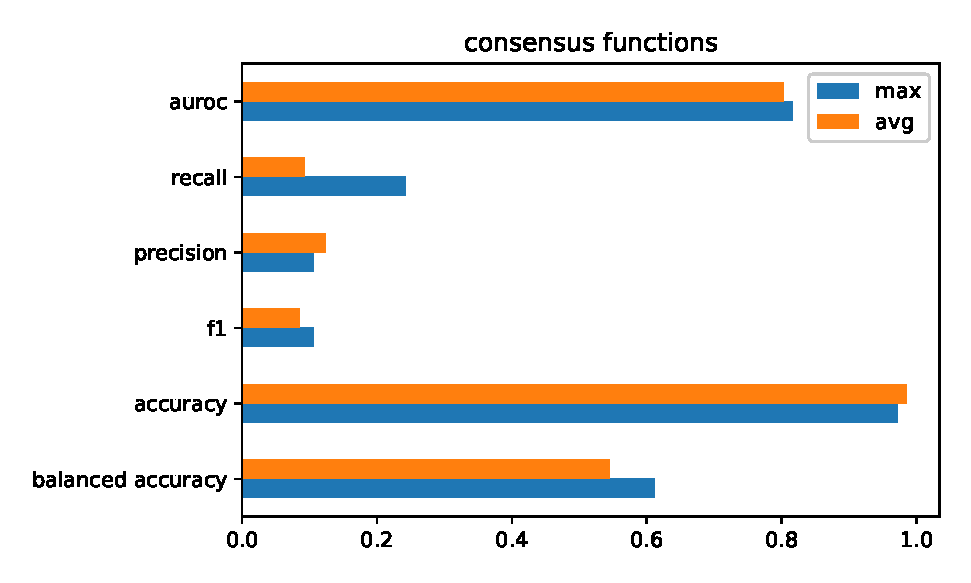
\includegraphics[width=0.7\textwidth, height=0.8\textwidth, keepaspectratio, interpolate]{img/07_consensus.eps}
    \caption{Vergleich von Max- und Avg-Aggregation am Test-Set (ir-CSN mit $\gamma_\tau = 2$) }
    \label{fig:consensus}
\end{figure}

Die Avg-Aggregation weist in allen Fällen eine knapp höhere Precision und Accuracy auf, während die Max-Aggregation einen deutlich höheren Recall, eine leicht höhere AUROC und Balanced Accuracy und in den meisten Fällen einen leicht höheren F1-Score.
Die Ergebnisse lassen sich zum Teil dadurch erklären, dass die Scores durch die Mittelung der Avg-Aggregation immer niedriger sind als die Scores in der Max-Aggregation, wodurch die Anzahl aller Positives insgesamt abnimmt.
Die Avg-Aggregation ist also deutlich sensibler gegenüber False Positives.

Dennoch wird die Avg-Aggregation als primäre Aggregation für den weiteren Verlauf festgelegt.
Zum einen, da die Metriken im Schnitt einen besseren Kompromiss darstellen.
Zum anderen, da sie die Realität logisch abbildet:
Enthält ein Clip von 10 Sekunden zwei Aktionen -- die eine Aktion ganz zu Beginn und die andere Aktion kurz vorm Ende, ist die erste Aktion nicht im letzten Chunk und die zweite Aktion nicht im ersten Chunk sichtbar.
Die Max-Aggregation kann derartige Zustände erkennen, da die Maxima sich auf die lokalen Stellen im Clip beziehen, während die Lokalität bei der Avg-Aggregation verwässert und ein hohes Maximum leicht durch weitere niedrige Scores überstimmt werden kann.

\begin{tcolorbox}[title=Todo]
    \begin{itemize}
        \item Grafik: besser als Ausschläge (Acc ist 5 \% besser in Avg als in Max..)
        \item ermittel Abfall der Metriken im Vergleich (val und test): Ist der Abfall insbesondere bei kleinen $\Delta$ größer?
    \end{itemize}
\end{tcolorbox}

\section{Evaluation der Experimente}

\begin{tcolorbox}[title=Todo]
    \begin{itemize}
        \item jeweils epochen und $\gls{tld:Theta}_\text{train}$ nennen
        \item Parallel coordinates
    \end{itemize}
\end{tcolorbox}


\subsubsection{Initialisierung und Hyperparameter Optimierung}

Um eine zeitliche Clip-Abdeckung von 3 bis 6 Sekunden pro Sample zu ermöglichen werden zu diesem Zweck in der zweiten Phase verschiedene Hyperparameter getestet.
Alle Modelle nutzen eine dynamisches Avg-\pool-Layer zwischen dem letzten \conv- und dem ersten \fc-Layer, das die Verarbeitung von Tensoren variabler Länge $T$ zulässt.
Um eine geeignete Methode zu finden, wird der Einfluss von Avg-Pooling und Subsampling auf den jeweils gleichen Daten pro Modell verglichen.
Zudem werden der Einfluss verschiedener Auflösungen verglichen.

\autoref{tab:pre} zeigt die Ergebnisse, indem pro Modell ausgehend von das Basiskonfiguration zunächst die Clip-Abdeckung und Anschließend die Auflösung erhöht wird.
Die Abdeckung wird durch die Erhöhung von $\gamma_t$, die Erhöhung von $\gamma_\tau$ oder der Erhöhung beider Parameter vergrößert.
Anschließend wird basierend auf dem besten Ergebnis testweise $\gamma_s$ erhöht.
Die Experimente in \autoref{tab:pre} wurden dazu mit $\gls{tld:Theta}_\text{train} = 100$ Samples pro Klasse (inklusive 100 Background-Samples) durchgeführt.

\begin{figure}
    \centering
    \csvreader[no head,tabular=|l|r|r|r|r||r|r|r|,
    table head=\hline,late after line=\\\hline]{tbl/pre-eval.csv}
    {1=\model,2=\s,3=\t,4=\sr,5=\d,6=\result,7=\ihatelatex,8=\reallyshittylatex}
    {\model & \s & \t & \sr & \d & \result & \ihatelatex & \reallyshittylatex}
    \caption{Ergebnisse zur Hyperparameter-Optimierung}
    \label{tab:pre}
\end{figure}

\subsubsection{Verifikation}

\begin{tcolorbox}[title=Todo]
    \begin{itemize}
        \item protokoll: Abbruchbedingung sinnvoll?
        \item beispiele im Anhang?,
        \item häufige fehler (Datenfehler, Klassifikationsfehler),
        \item basis: beste ep
        \item Anzahl = 25 ?
    \end{itemize}
\end{tcolorbox}


In der dritten Phase werden diejenigen Samples, die den größen Loss innerhalb eines Trainings vorweisen, genauer analysiert.
Grundlage ist eine Analyse der Experimente aus Phase 2.
In Zuge der Analyse werden zum einen Datenfehler (wie in \autoref{sec:nachgang} beschrieben) behoben.
Zusätzlich werden manuell Informationen über die $25$ größten Fehler (abhängig vom Loss im Fehlerreport) innerhalb eines Experiments erhoben.

Die Analyse folgt einem definiertem Protokoll:
Sind alle Experimente einer Phase abgeschlossen, wird zunächst eine neue Transaktionsdatei erstellt.
Für jedes der genannten Durchläufe (der jeweiligen Phase) wird das Relabel-Tool mit den persistierten Score- und Loss-Werte des je letzten Epoche initialisiert.
Das Relabel-Tool erhält ebenfalls Zugriff auf die Datenbankinstanz, die sich aus der persistierten JSON-Datenbank und den in dieser Phase bereits durchgeführten Transaktionen zusammensetzt.
So kann das Relabel-Tool \ua erkennen, das der selbe Fehler schon in einem vorherigen Experiment behoben wurde.

Die Samples werden absteigend nach Loss-Wert sortiert und dem Nutzer iterativ präsentiert.
Der Nutzer kann das Sample als Datenfehler in Form einer Transaktion beheben oder als Klassifikationsfehler markieren.
Als Klassifikationsfehler markierte Samples werden automatisch geloggt und im Cloud-Speicher abgelegt.
Die Analyse kann abgebrochen werden, sobald mindestens $25$ Klassifikationsfehler erfasst wurden.

\subsubsection{Fine-Tuning und Benchmark}

\begin{tcolorbox}[title=Todo]
    \begin{itemize}
        \item anpassung pro modell: reaktiv auf Phänome, wie Overfitting, Optimierung pro Modell (Anzahl Epochen, Weight Decay, Tiefere Modelle)?
    \end{itemize}
\end{tcolorbox}

In der vierten Phase werden die besten Modelle aus Phase 2 mit bis zu $\gls{tld:Theta}_\text{train} = 250$ Samples pro Klasse auf Grundlage der verifizierten Datenbank aus Phase 3 nachtrainiert.
Anschließend wird reaktiv auf die Ergebnisse des Trainings reagiert.
\autoref{tab:exp4} zeigt die Ergebnisse.

\begin{figure}
    \centering
    \csvreader[no head,tabular=|l||r|r|r||r|r|r|,
    table head=\hline,late after line=\\\hline]{tbl/exp_phase_4.csv}
    {1=\model,2=\s,3=\t,4=\sr,5=\d,6=\result,7=\ihatelatex}
    {\model & \s & \t & \sr & \d & \result & \ihatelatex}
    \caption{Ergebnisse zur Fine-Tuning}
    \label{tab:exp4}
\end{figure}


\section{Kategorisierung der Aktionsklassen}

\begin{tcolorbox}[title=Todo]
    \begin{itemize}
        \item Idee: pca und clustering in vier gruppen
        \item Vergleich der Evaluation auf subsets (SOCC-HAR-8, -16, -24, -32)
        \item Optional: SOCC-HAR-NET, SOCC-HAR-DB Klassen
    \end{itemize}
\end{tcolorbox}

Da ein Großteil der in \autoref{subsec:metriken} vorgestellten Metriken pro Klasse erhoben werden, kann eine genauere Analyse über die Komplexität zur Klassifizierung einer einzelnen Klasse gemacht werden.
Wie einfach oder schwer eine Klasse zu lernen ist, soll pro Modell und Modell-übergreifend veranschaulicht werden.

\subsection*{Vergleich mit Klassen aus SoccerNet, SoccerDB}

\section{Grenzen und Hypothesen}

\begin{tcolorbox}[title=Todo]
    Desweiteren sind bis auf AUROC alle Metriken durch einen Score-Grenzwert definiert, der angibt ab welcher Sicherheit ein Label für einen Score-Wert übernommen wird.
    Initial liegt der Grenzwert bei 50 \%.
    Wenn der Label-Score eines Samples über 50 \% liegt, wird es \ua mit diesem Label klassifiziert.
    Es kann entweder ein globaler Score-Grenzwert für alle Labels oder individuelle Grenzwerte pro Label gesetzt werden.
    Um einen geeigneten globalen Score-Wert zu finden werden vorab verschiedene Grenzwerte (an Balanced Accuracy) ausprobiert, der für alle weiteren Metriken verwendet wird.
\end{tcolorbox}

% \section{Grenzen und Hypothesen}

%\section{Anwendung der Modelle auf SoccerNet-500}
%\label{sec:anwendung-der-modelle-auf-soccernet-500}

%Im ersten Durchgang werden alle Modelle mit Daten aus SoccerNet-500 trainiert.

%Die Daten werden wie im Original-Paper nach Spiel aufgeteilt im Verhältnis (3:2:1).
%Für jede Annotation wird ein Eintrag im Datenframe erstellt, sowie für jede Spielminute, in der keine der drei definierten Aktionen stattfindet.
%Während in SoccerNet das ganze Videomaterial von einer Minute komprimiert wurde, werden in diesem Aufbau nur Tensoren von 5 Sekunden als Input genutzt.
%Für die Spielminuten ohne Annotation wird eine Hintergrund-Aktion in der 30. Sekunde der Spielminute erstellt, sodass es zu keiner potenziellen Überschneidung kommen kann.

%Aus dem Datenframe werden anschließend H5-Datensets mit je 400 (50 und 100) Trainings- (Validierungs- und Test-) samples pro Klasse gespeichert.

%\subsection{Ergebnisse}

%<<tab:soccernet>> zeigt die Ergebnisse des ersten Durchlaufs.

%\begin{figure}
%    \centering
%    \csvautotabular{tbl/s.csv}
%    \caption[]{Vergleich SoccerNet Benchmark}
%    \label{tab:soccernet}
%\end{figure}

%In alle Modellen wurden nur die hinteren \fc-, sowie Teile des letzten \res-Layers trainiert, sodass die Zahl der trainierbaren Parameter etwa gleich sind pro Modell.
%Weitere Layer wurden bewusst nicht trainiert, um ein Overfitting zu vermeiden.
%Für alle Modelle gilt, dass sie ab einer gewissen Epoche overfitten, was auf zu wenig Samples zurückzuführen ist.
%Insbesondere ip-CSN ist schwer zu trainieren, da es aufgrund der hohen Auflösung viel Speicher einnimmt und somit nur eine kleine Batchgröße ermöglicht.
%Im Gegenseatz zu Slowfast, das die selbe Auflösung verarbeitet, werden in ip-CSN alle Frames des Tensors verarbeitet (in Slowfast nur jeder zweite).
